\documentclass[leqno]{article}
\usepackage[utf8]{inputenc}
\usepackage{enumitem}
\usepackage{tikz}
\usepackage[parfill]{parskip} % Don't start new paragraph with tab.
\usepackage{amsmath} % For \tag and \eqref

\title{Computationele logica}
\author{
    Kamans, Jim\\
    \texttt{10302905}
    \and
    Roosingh, Sander\\
    \texttt{11983957}
    \and
    Schenk, Stefan\\
    \texttt{11881798}
}
\date{November 2017}

\begin{document}

\maketitle

\section{Exercise 1}

$\phi$ = the date of Cheryl's birthday, a = Albert, b = Bernard, c = Cheryl \\
\\
With arrows we are representing the children’s knowledge relations, so we’ll get an epistemic model: all relations R1, R2, R3 are equivalence relations. So in particular they are reflexive, but for simplicity of drawing we skipped the loops.
\\

\begin{enumerate}[label=(\alph*)]
    \item Model M of the situation immediately after Cheryl gives the boys their pieces of information: \\

    \begin{center}
    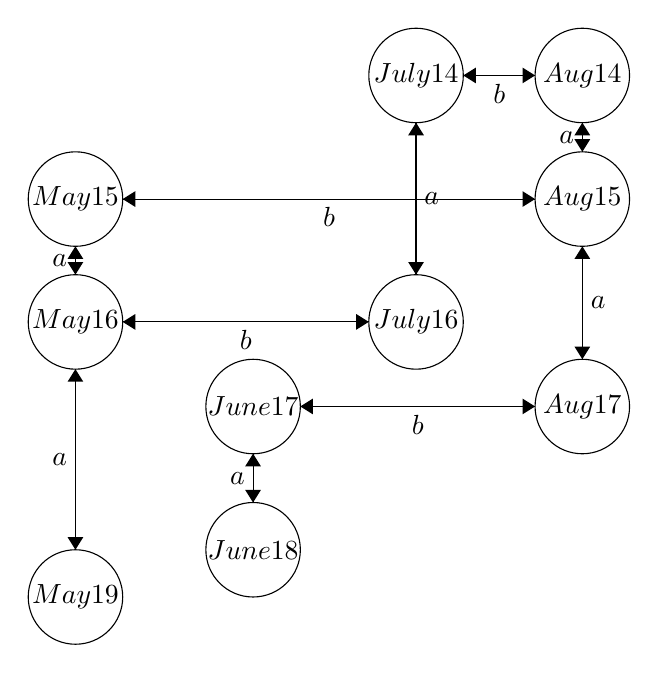
\begin{tikzpicture}[scale=0.2]
    \tikzstyle{every node}+=[inner sep=0pt]
    \draw [black] (9.383,-12.68) circle (3);
    \draw (9.38,-12.68) node {$May15$};
    \draw [black] (20.663,-25.854) circle (3);
    \draw (20.66,-25.85) node {$June17$};
    \draw [black] (9.383,-20.483) circle (3);
    \draw (9.38,-20.48) node {$May16$};
    \draw [black] (9.383,-37.949) circle (3);
    \draw (9.38,-37.95) node {$May19$};
    \draw [black] (20.663,-34.949) circle (3);
    \draw (20.66,-34.95) node {$June18$};
    \draw [black] (31.01,-20.483) circle (3);
    \draw (31.01,-20.48) node {$July16$};
    \draw [black] (31.01,-4.832) circle (3);
    \draw (31.01,-4.83) node {$July14$};
    \draw [black] (41.568,-4.832) circle (3);
    \draw (41.57,-4.83) node {$Aug14$};
    \draw [black] (41.568,-12.68) circle (3);
    \draw (41.57,-12.68) node {$Aug15$};
    \draw [black] (41.568,-25.854) circle (3);
    \draw (41.57,-25.85) node {$Aug17$};
    \draw [black] (12.38,-20.48) -- (28.01,-20.48);
    \fill [black] (28.01,-20.48) -- (27.21,-19.98) -- (27.21,-20.98);
    \draw (20.2,-20.98) node [below] {$b$};
    \draw [black] (12.38,-12.68) -- (38.57,-12.68);
    \fill [black] (38.57,-12.68) -- (37.77,-12.18) -- (37.77,-13.18);
    \draw (25.48,-13.18) node [below] {$b$};
    \draw [black] (34.01,-4.83) -- (38.57,-4.83);
    \fill [black] (38.57,-4.83) -- (37.77,-4.33) -- (37.77,-5.33);
    \draw (36.29,-5.33) node [below] {$b$};
    \draw [black] (23.66,-25.85) -- (38.57,-25.85);
    \fill [black] (38.57,-25.85) -- (37.77,-25.35) -- (37.77,-26.35);
    \draw (31.12,-26.35) node [below] {$b$};
    \draw [black] (28.01,-20.48) -- (12.38,-20.48);
    \fill [black] (12.38,-20.48) -- (13.18,-20.98) -- (13.18,-19.98);
    \draw [black] (38.57,-12.68) -- (12.38,-12.68);
    \fill [black] (12.38,-12.68) -- (13.18,-13.18) -- (13.18,-12.18);
    \draw [black] (38.57,-25.85) -- (23.66,-25.85);
    \fill [black] (23.66,-25.85) -- (24.46,-26.35) -- (24.46,-25.35);
    \draw [black] (38.57,-4.83) -- (34.01,-4.83);
    \fill [black] (34.01,-4.83) -- (34.81,-5.33) -- (34.81,-4.33);
    \draw [black] (20.66,-28.85) -- (20.66,-31.95);
    \fill [black] (20.66,-31.95) -- (21.16,-31.15) -- (20.16,-31.15);
    \draw (20.16,-30.4) node [left] {$a$};
    \draw [black] (20.66,-31.95) -- (20.66,-28.85);
    \fill [black] (20.66,-28.85) -- (20.16,-29.65) -- (21.16,-29.65);
    \draw [black] (9.38,-23.48) -- (9.38,-34.95);
    \fill [black] (9.38,-34.95) -- (9.88,-34.15) -- (8.88,-34.15);
    \draw (8.88,-29.22) node [left] {$a$};
    \draw [black] (9.38,-34.95) -- (9.38,-23.48);
    \fill [black] (9.38,-23.48) -- (8.88,-24.28) -- (9.88,-24.28);
    \draw [black] (9.38,-17.48) -- (9.38,-15.68);
    \fill [black] (9.38,-15.68) -- (8.88,-16.48) -- (9.88,-16.48);
    \draw [black] (9.38,-15.68) -- (9.38,-17.48);
    \fill [black] (9.38,-17.48) -- (9.88,-16.68) -- (8.88,-16.68);
    \draw (8.88,-16.58) node [left] {$a$};
    \draw [black] (31.01,-7.83) -- (31.01,-17.48);
    \fill [black] (31.01,-17.48) -- (31.51,-16.68) -- (30.51,-16.68);
    \draw [black] (31.01,-17.48) -- (31.01,-7.83);
    \fill [black] (31.01,-7.83) -- (30.51,-8.63) -- (31.51,-8.63);
    \draw (31.51,-12.66) node [right] {$a$};
    \draw [black] (41.57,-9.68) -- (41.57,-7.83);
    \fill [black] (41.57,-7.83) -- (41.07,-8.63) -- (42.07,-8.63);
    \draw [black] (41.57,-7.83) -- (41.57,-9.68);
    \fill [black] (41.57,-9.68) -- (42.07,-8.88) -- (41.07,-8.88);
    \draw (41.07,-8.76) node [left] {$a$};
    \draw [black] (41.57,-15.7) -- (41.57,-22.85);
    \fill [black] (41.57,-22.85) -- (42.07,-22.05) -- (41.07,-22.05);
    \draw [black] (41.57,-22.85) -- (41.57,-15.68);
    \fill [black] (41.57,-15.68) -- (41.07,-16.48) -- (42.07,-16.48);
    \draw (42.07,-19.27) node [right] {$a$};
    \end{tikzpicture}
    \end{center}

    \item Epistemic sentence encoding Albert's first announcement: \\
    \\
    $!_a (\neg K_a \phi \wedge K_a \neg K_b \phi)$ \\
    \\
    Albert announces that he doesn't know the date of Cheryl's birthday, and that he knows that Bernard doesn't know the date of Cheryl's birthday either.
    \\

    \item Updated model M' after Albert's first announcement: \\
    \\
    If Bernard either knew that the date was the 19th of May or the 18th of June, he would've instantly known the date of Cheryl's birthday because no other dates exists with these day numbers. Therefore, May and June are no longer an option after the public announcement.
    \\

    \begin{center}
    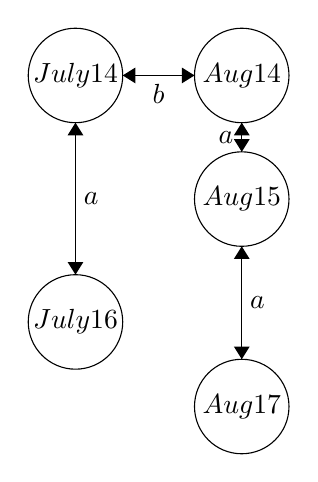
\begin{tikzpicture}[scale=0.2]
    \tikzstyle{every node}+=[inner sep=0pt]
    \draw [black] (31.01,-20.483) circle (3);
    \draw (31.01,-20.48) node {$July16$};
    \draw [black] (31.01,-4.832) circle (3);
    \draw (31.01,-4.83) node {$July14$};
    \draw [black] (41.568,-4.832) circle (3);
    \draw (41.57,-4.83) node {$Aug14$};
    \draw [black] (41.568,-12.68) circle (3);
    \draw (41.57,-12.68) node {$Aug15$};
    \draw [black] (41.568,-25.854) circle (3);
    \draw (41.57,-25.85) node {$Aug17$};
    \draw [black] (34.01,-4.83) -- (38.57,-4.83);
    \fill [black] (38.57,-4.83) -- (37.77,-4.33) -- (37.77,-5.33);
    \draw (36.29,-5.33) node [below] {$b$};
    \draw [black] (38.57,-4.83) -- (34.01,-4.83);
    \fill [black] (34.01,-4.83) -- (34.81,-5.33) -- (34.81,-4.33);
    \draw [black] (31.01,-7.83) -- (31.01,-17.48);
    \fill [black] (31.01,-17.48) -- (31.51,-16.68) -- (30.51,-16.68);
    \draw [black] (31.01,-17.48) -- (31.01,-7.83);
    \fill [black] (31.01,-7.83) -- (30.51,-8.63) -- (31.51,-8.63);
    \draw (31.51,-12.66) node [right] {$a$};
    \draw [black] (41.57,-9.68) -- (41.57,-7.83);
    \fill [black] (41.57,-7.83) -- (41.07,-8.63) -- (42.07,-8.63);
    \draw [black] (41.57,-7.83) -- (41.57,-9.68);
    \fill [black] (41.57,-9.68) -- (42.07,-8.88) -- (41.07,-8.88);
    \draw (41.07,-8.76) node [left] {$a$};
    \draw [black] (41.57,-15.7) -- (41.57,-22.85);
    \fill [black] (41.57,-22.85) -- (42.07,-22.05) -- (41.07,-22.05);
    \draw [black] (41.57,-22.85) -- (41.57,-15.68);
    \fill [black] (41.57,-15.68) -- (41.07,-16.48) -- (42.07,-16.48);
    \draw (42.07,-19.27) node [right] {$a$};
    \end{tikzpicture}
    \end{center}

    \item Epistemic sentence and updated model M'' after Bernard's announcement: \\
    \\
    $!_b (K_b \phi)$ \\
    \\
    Bernard announces that he knows the date of Cheryl's birthday now.
    \\
    \begin{center}
    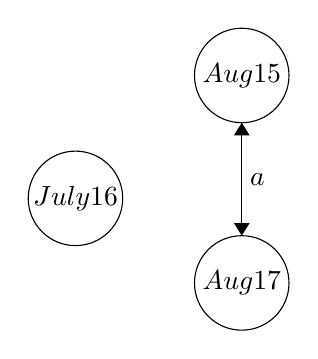
\begin{tikzpicture}[scale=0.2]
    \tikzstyle{every node}+=[inner sep=0pt]
    \draw [black] (31.01,-20.483) circle (3);
    \draw (31.01,-20.48) node {$July16$};
    \draw [black] (41.568,-12.68) circle (3);
    \draw (41.57,-12.68) node {$Aug15$};
    \draw [black] (41.568,-25.854) circle (3);
    \draw (41.57,-25.85) node {$Aug17$};
    \draw [black] (41.57,-15.7) -- (41.57,-22.85);
    \fill [black] (41.57,-22.85) -- (42.07,-22.05) -- (41.07,-22.05);
    \draw [black] (41.57,-22.85) -- (41.57,-15.68);
    \fill [black] (41.57,-15.68) -- (41.07,-16.48) -- (42.07,-16.48);
    \draw (42.07,-19.27) node [right] {$a$};
    \end{tikzpicture}
    \end{center}

    \item Epistemic sentence and updated model M''' after Albert's second announcement: \\
    \\
    $!_a (K_a \phi)$ \\
    \\
    Albert announces that he too knows.
    \\
    \begin{center}
    
\begin{tikzpicture}[scale=0.2]
    \tikzstyle{every node}+=[inner sep=0pt]
    \draw [black] (31.01,-20.483) circle (3);
    \draw (31.01,-20.48) node {$July16$};
    \end{tikzpicture}
    \end{center}

\end{enumerate}

\section{Exercise 2}
Prove formally that, for every sentence \(\varphi\), the sentence
\[\neg K_{a}\varphi \Rightarrow K_{a}\neg K_{a}\varphi\]
(expressing ``Negative Introspection of Knowledge'') is \textit{valid} on (the family of all) \textbf{epistemic} models.

Let $M = \{W, R_a, R_b, \dots, \nu\}$ be any epistemic model and let $w \in W$ be any world in it.

To prove the claim, suppose that $\neg K_a \varphi$ is true at $w$, i.e.
\begin{equation}
	\tag{1} \label{eq:ex2_1}
	w \models_M \neg K_a \varphi.
\end{equation}
We need to prove that
\begin{equation}
	\tag{?} \label{eq:ex2_?}
	w \models_M K_a \neg K_a \varphi.
\end{equation}
Let $v$ be an arbitrary world such that $w R_a v$.
By the semantics of $K_a$, \eqref{eq:ex2_1} implies

\section{Exercise 3}
Using the semantics of knowledge \(K_{a}\) and common knowledge \(Ck\), show that the following is NOT valid on \textit{epistemic models with (only) 2 agents a and b:}

\[(K_{a}K_{b}\phi\wedge K_{b}K_{a}\psi) \Rightarrow Ck(\phi\wedge\psi)\]
\\
$*$ = The representation of the world \\
P = $ \phi $ \\
Q = $ \psi $ \\
a = Albert, b = Bernard, c = Cheryl \\
\\
The epistemic model holds the beliefs that both a and b know P and Q, but they are not sure whether they know the fact that both a and b know P and Q.

\begin{center}
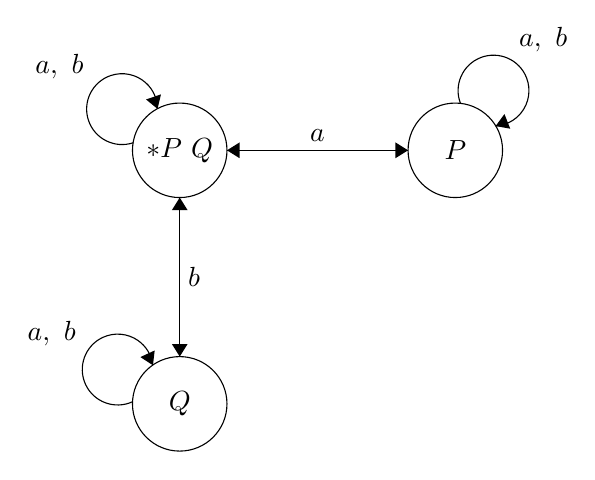
\begin{tikzpicture}[scale=0.2]
\tikzstyle{every node}+=[inner sep=0pt]
\draw [black] (13.5,-10.1) circle (3);
\draw (13.5,-10.1) node {$* P\mbox{ }Q$};
\draw [black] (31,-10.1) circle (3);
\draw (31,-10.1) node {$P$};
\draw [black] (13.5,-26.2) circle (3);
\draw (13.5,-26.2) node {$Q$};
\draw [black] (13.5,-13.1) -- (13.5,-23.2);
\fill [black] (13.5,-23.2) -- (14,-22.4) -- (13,-22.4);
\draw [black] (16.7,-10.1) -- (28,-10.1);
\fill [black] (28,-10.1) -- (27.2,-9.6) -- (27.2,-10.6);
\draw [black] (13.5,-23.2) -- (13.5,-13.1);
\fill [black] (13.5,-13.1) -- (13,-13.9) -- (14,-13.9);
\draw (14,-18.15) node [right] {$b$};
\draw [black] (28,-10.1) -- (16.5,-10.1);
\fill [black] (16.5,-10.1) -- (17.3,-10.6) -- (17.3,-9.6);
\draw (22.25,-9.6) node [above] {$a$};
\draw [black] (10.551,-9.619) arc (288.46232:0.46232:2.25);
\draw (7.42,-4.8) node [left] {$a,\mbox{ }b$};
\fill [black] (12.09,-7.47) -- (12.31,-6.55) -- (11.36,-6.87);
\draw [black] (31.331,-7.13) arc (201.38076:-86.61924:2.25);
\draw (36.58,-3.91) node [above] {$a,\mbox{ }b$};
\fill [black] (33.56,-8.56) -- (34.49,-8.73) -- (34.12,-7.8);
\draw [black] (10.515,-26.06) arc (295.04488:7.04488:2.25);
\draw (6.93,-21.73) node [left] {$a,\mbox{ }b$};
\fill [black] (11.8,-23.75) -- (11.91,-22.81) -- (11,-23.23);
\end{tikzpicture}
\end{center}

\end{document}


